\begin{figure}[!t]
\centering
\begin{subfigure}{0.32\textwidth}
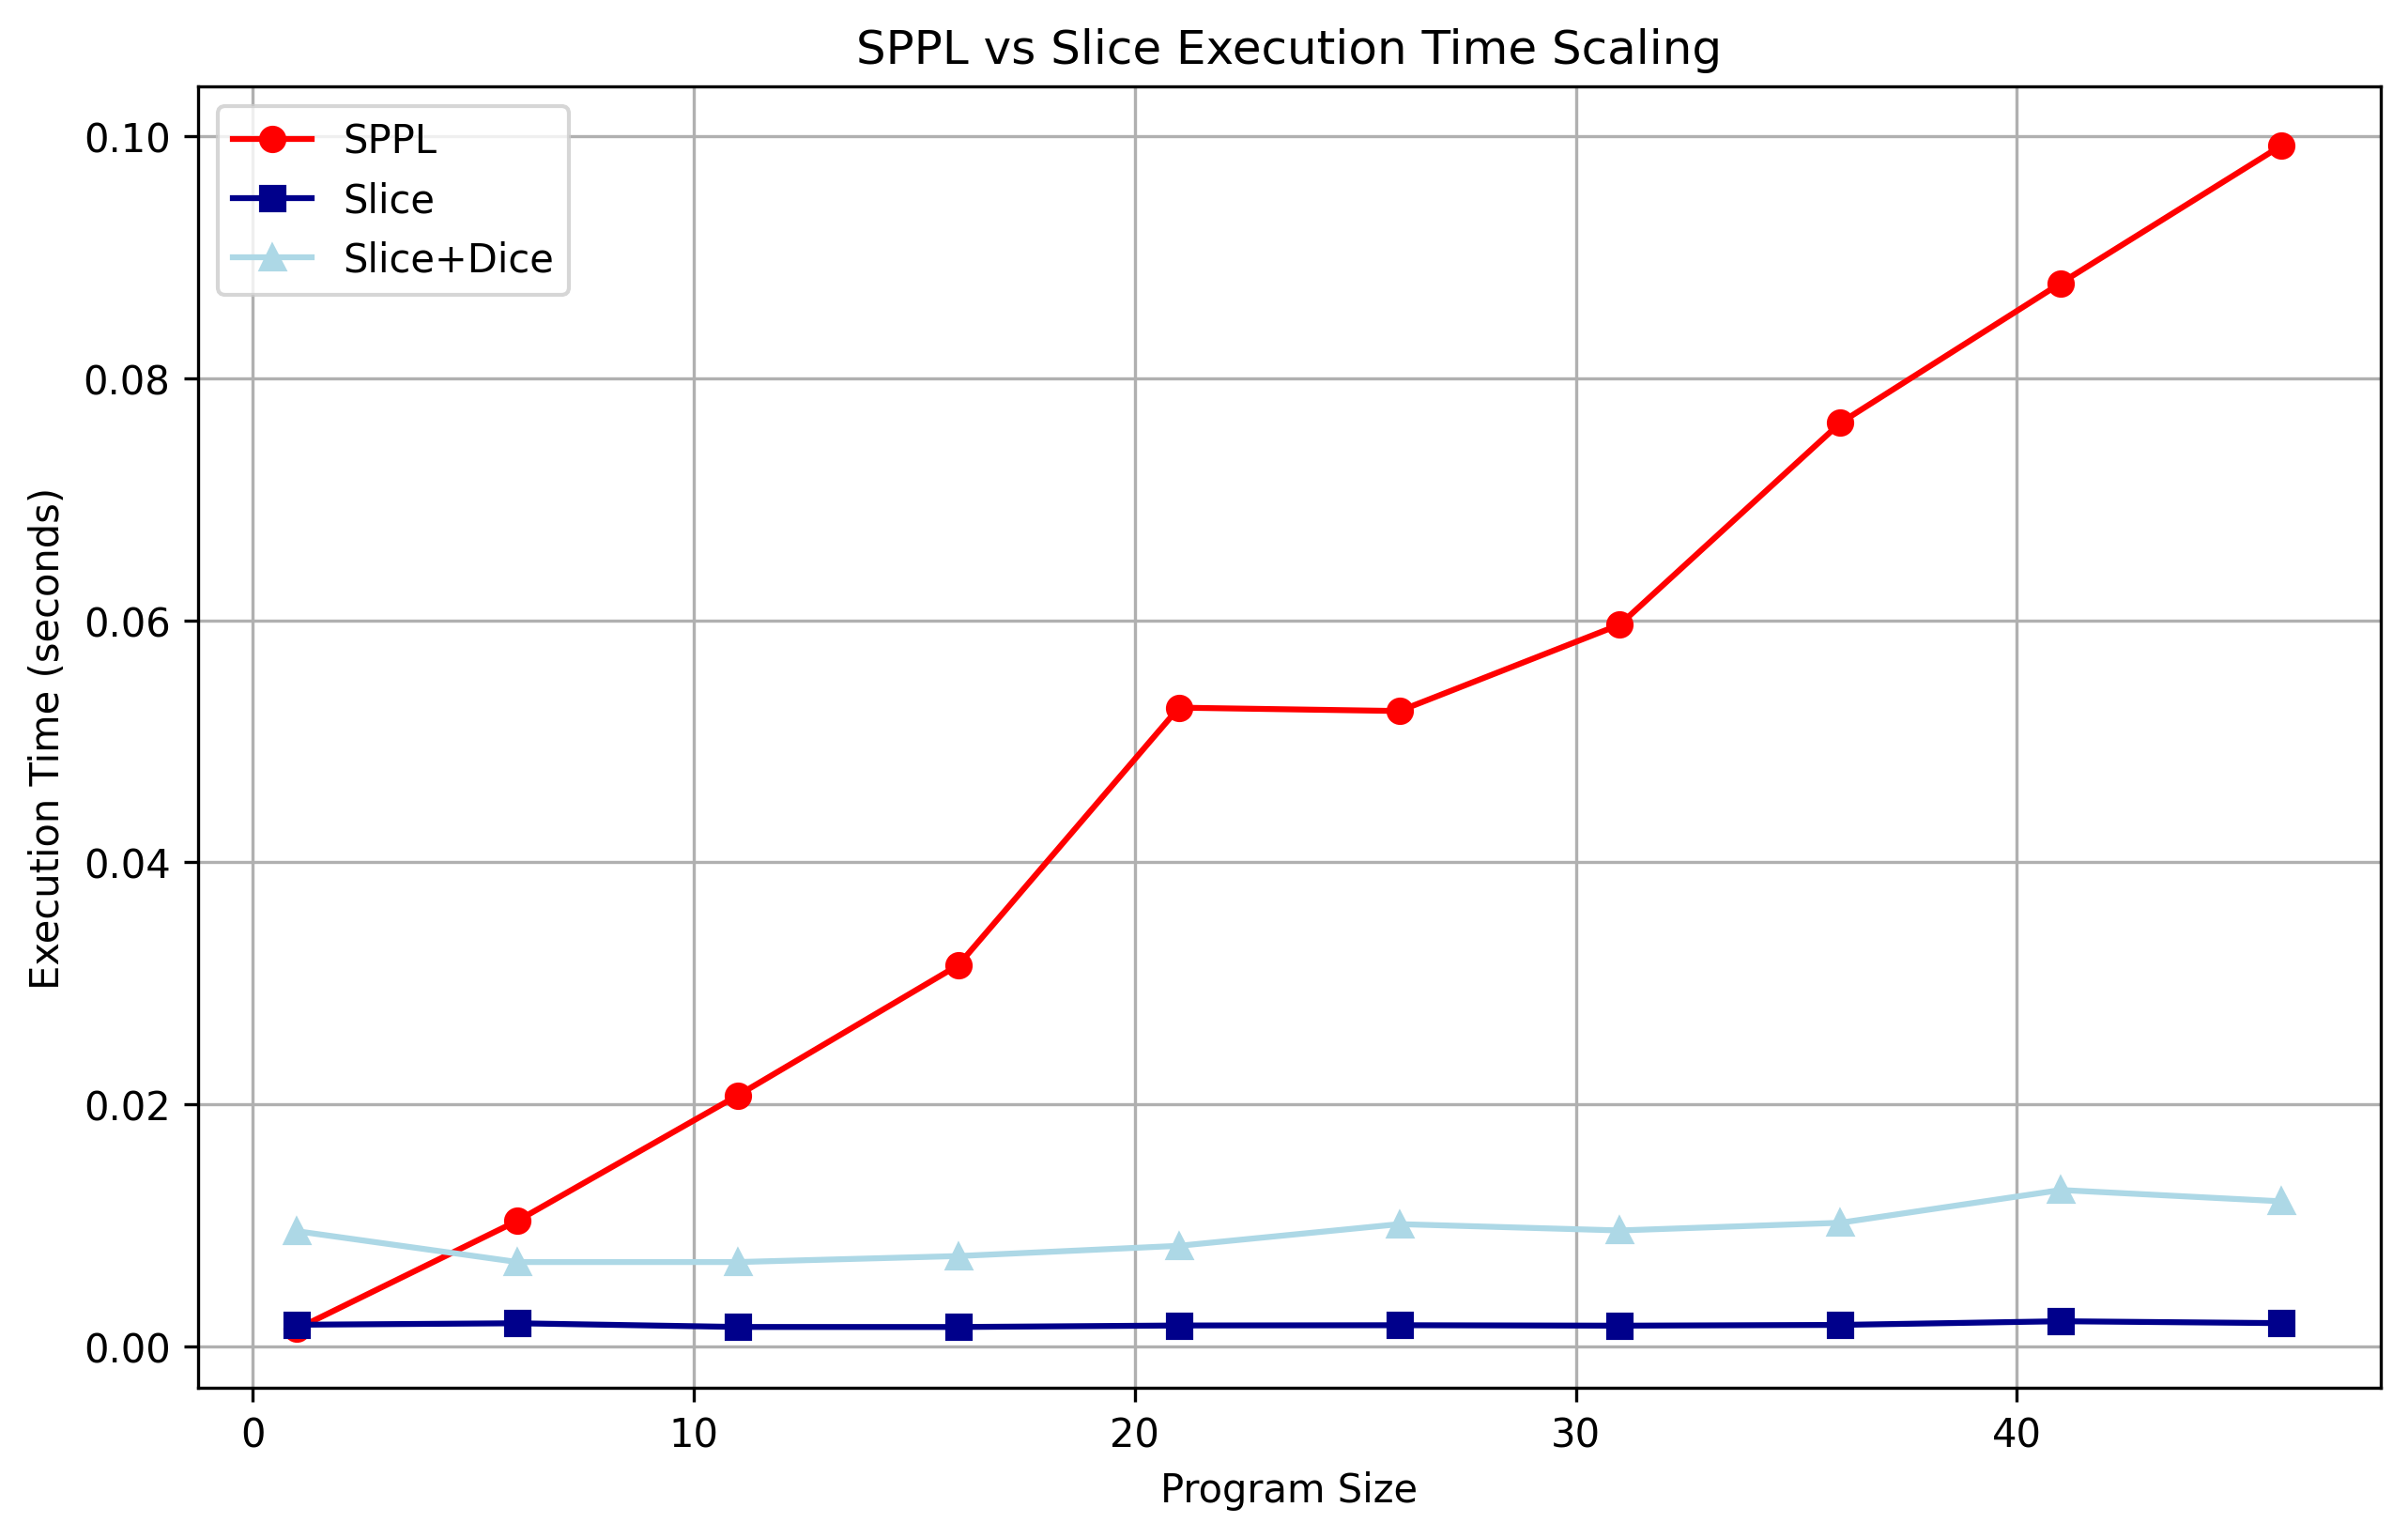
\includegraphics[width=\textwidth]{../images/scaling/build_conditional_independent_slice.png}
\caption{Conditional Independent}
\label{fig:cond-benchmarks-a}
\end{subfigure}
\hfill
\begin{subfigure}{0.32\textwidth}
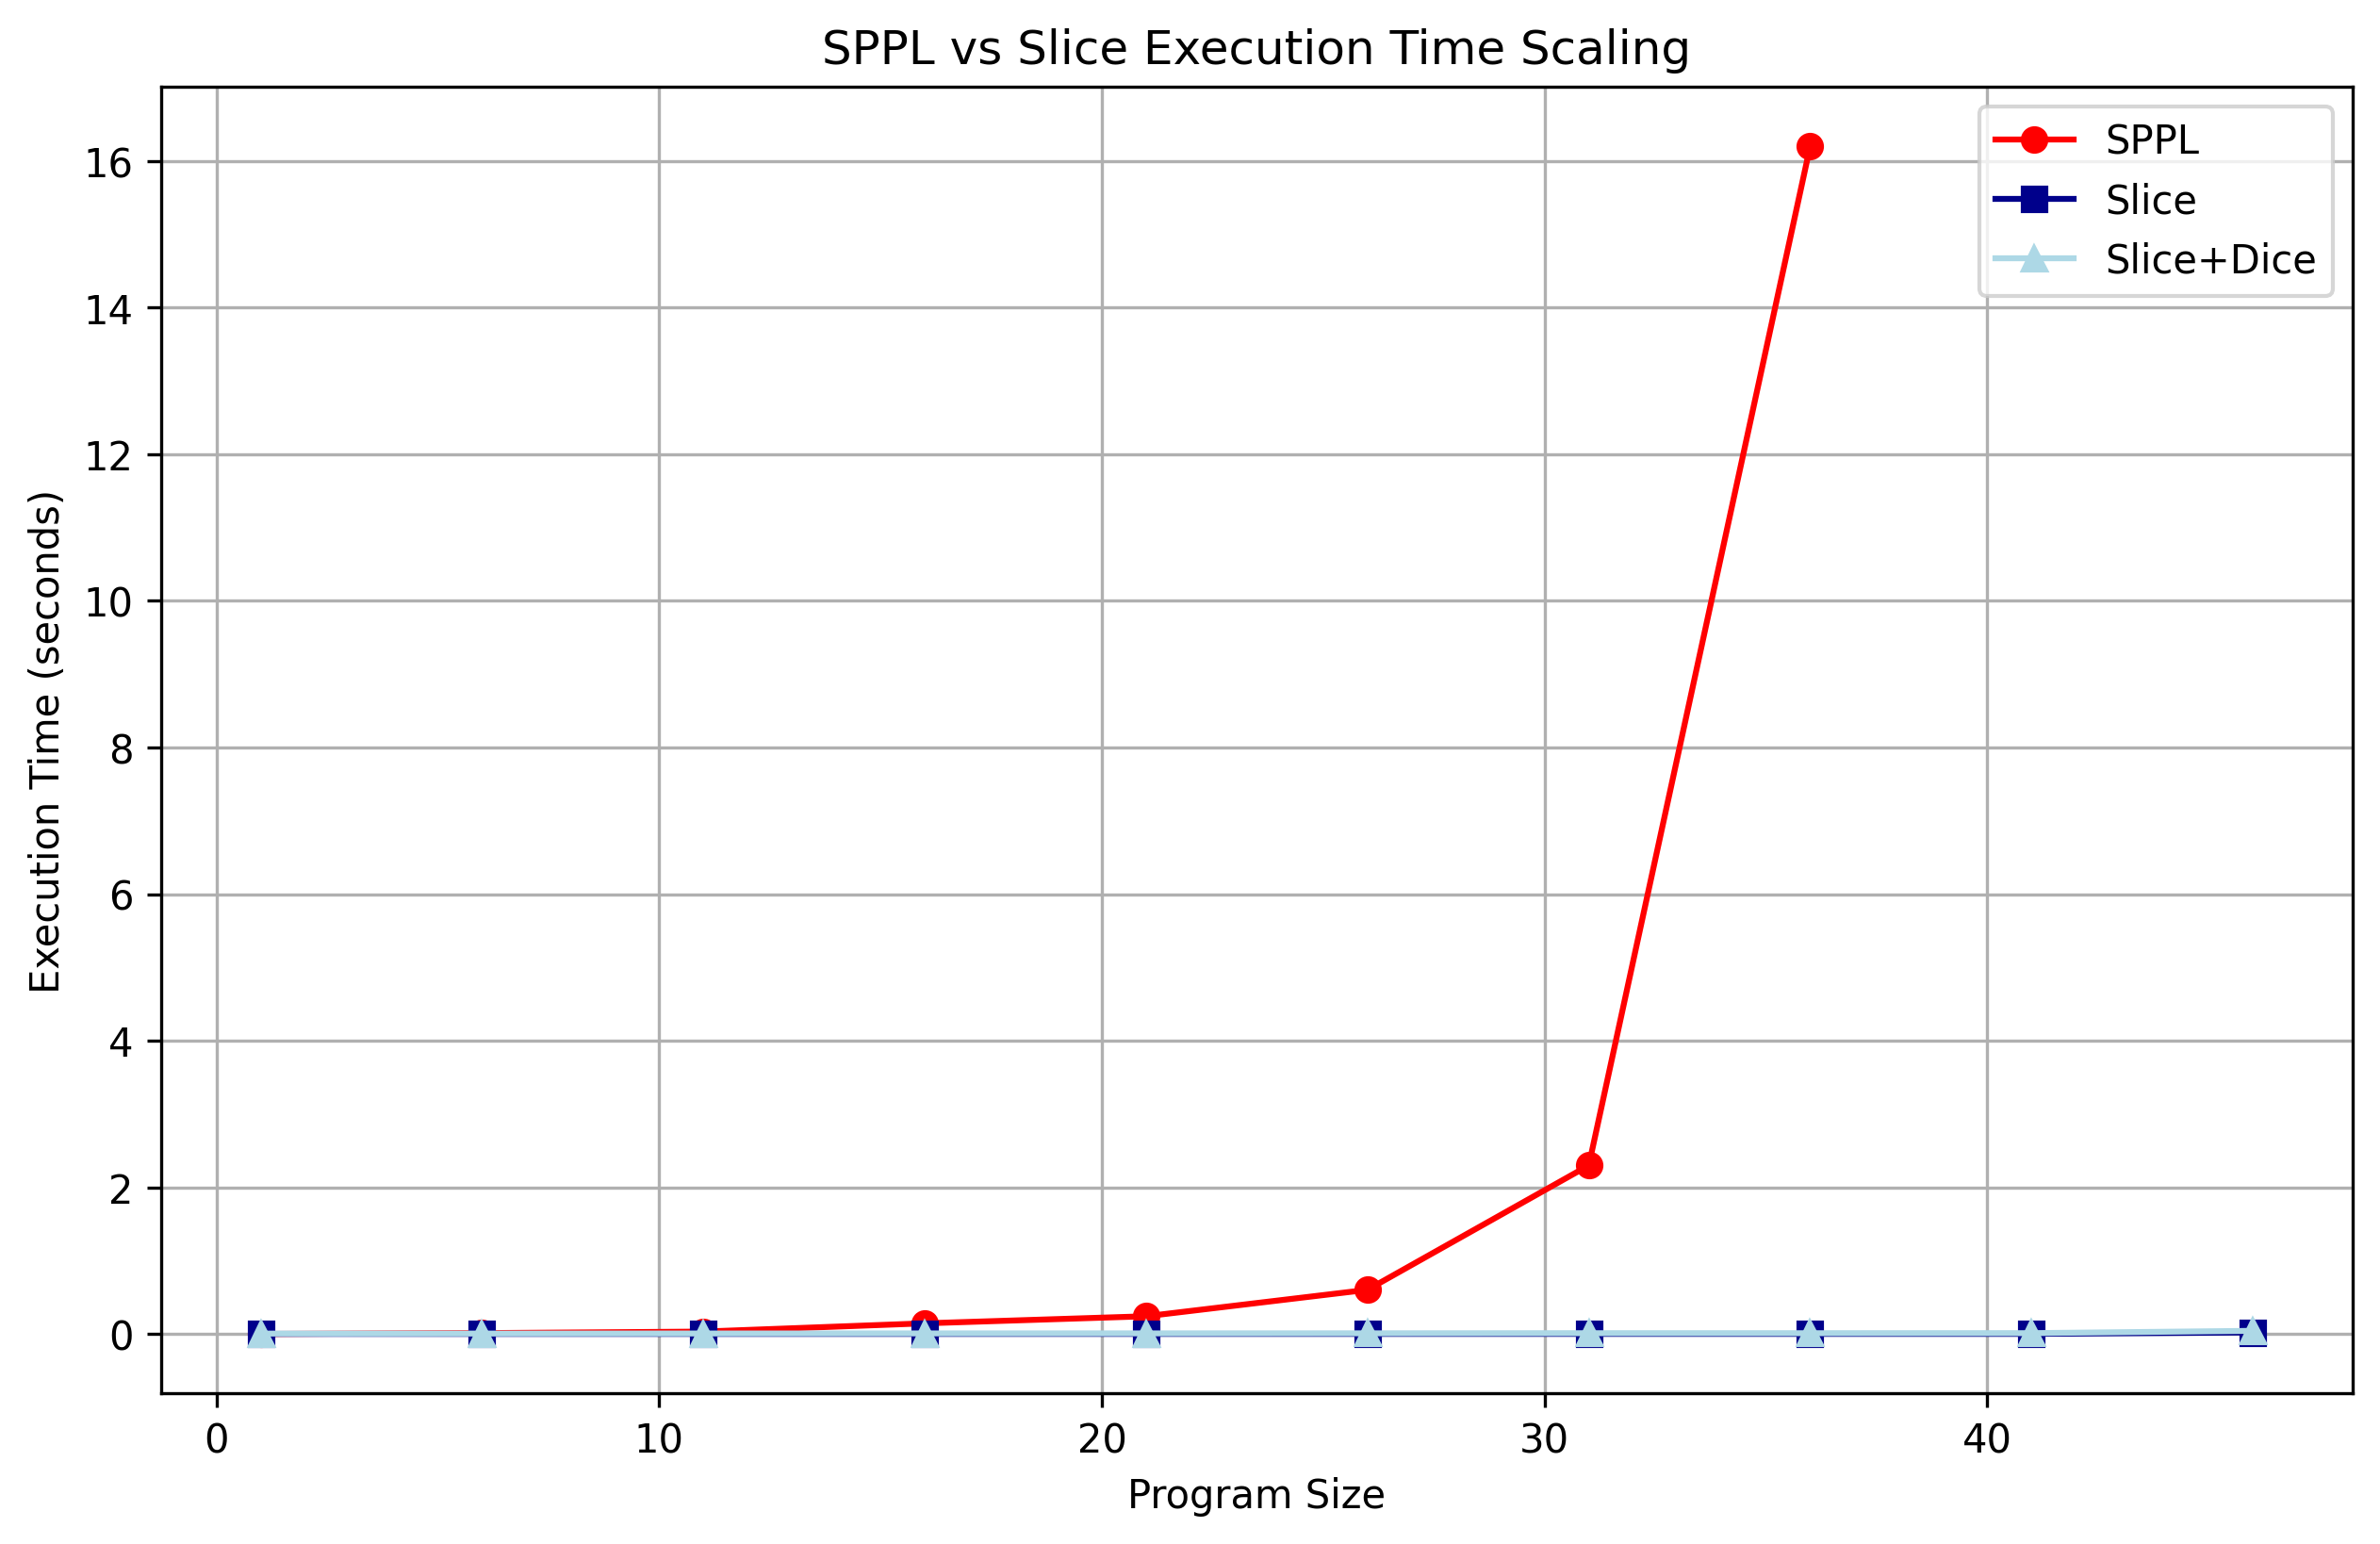
\includegraphics[width=\textwidth]{../images/scaling/build_conditional_random_independent_slice_1.png}
\caption{Conditional Random 1}
\label{fig:cond-benchmarks-b}
\end{subfigure}
\hfill
\begin{subfigure}{0.32\textwidth}
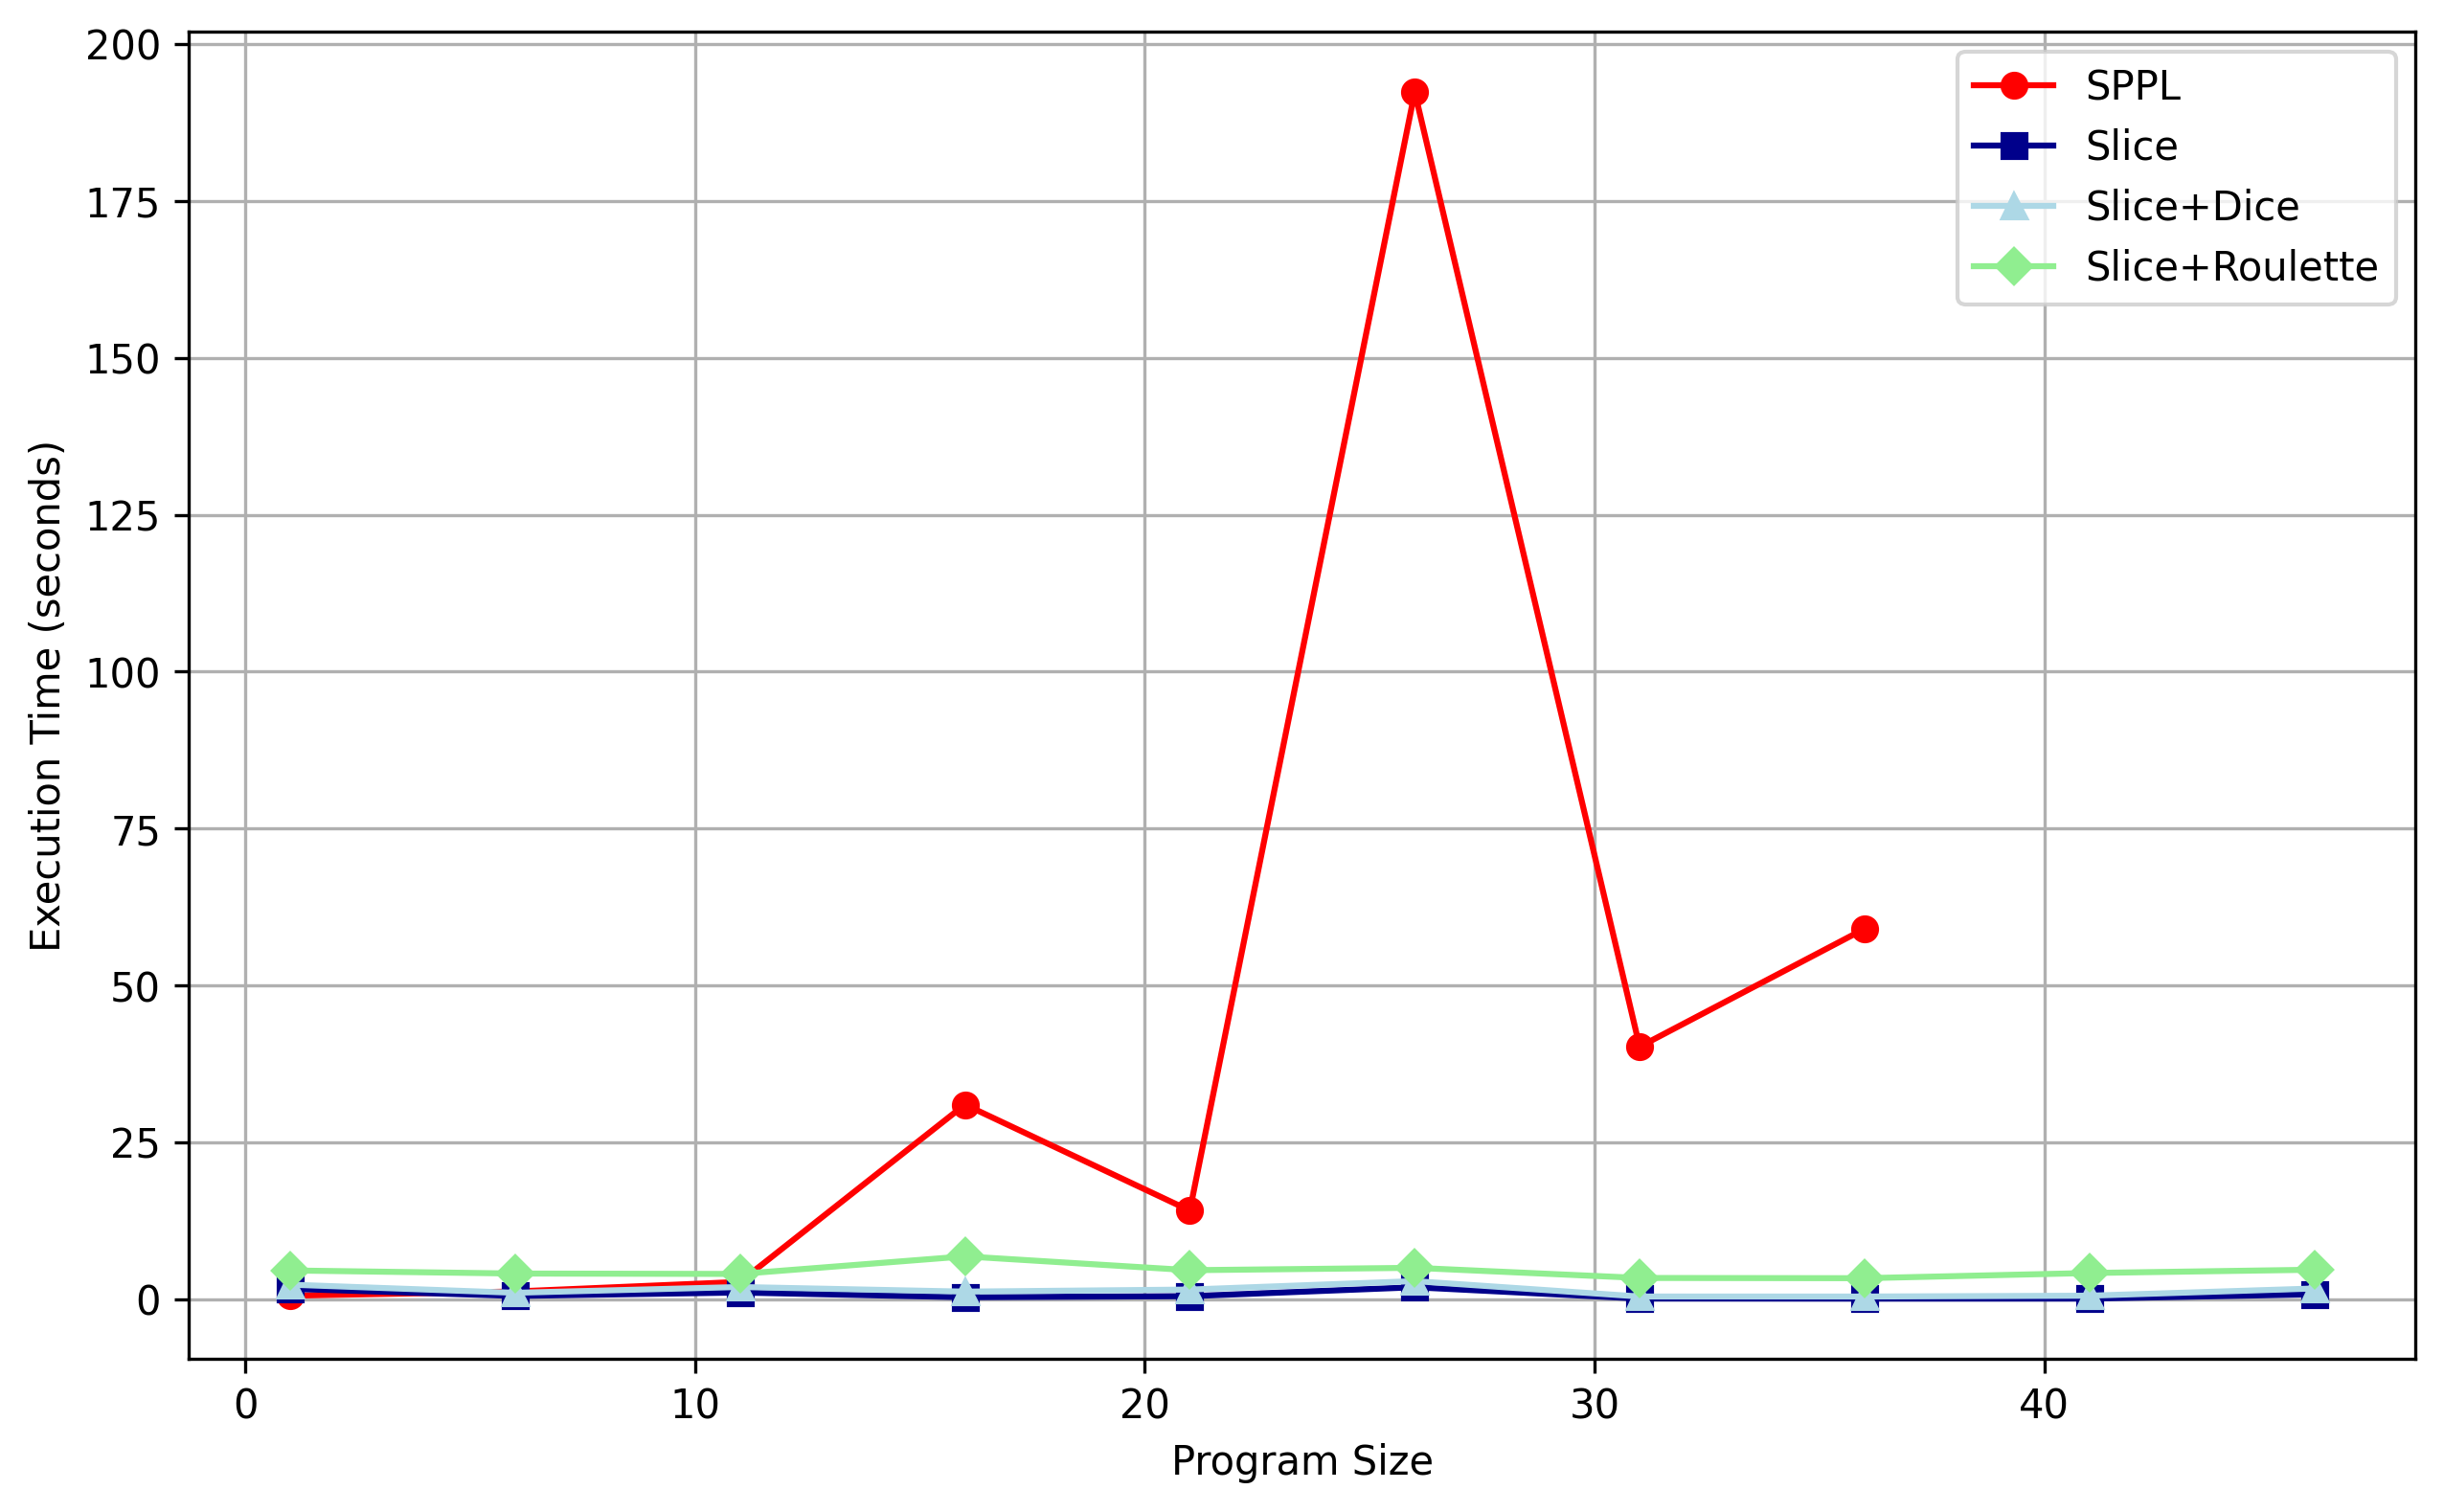
\includegraphics[width=\textwidth]{../images/scaling/build_conditional_random_independent_slice_2.png}
\caption{Conditional Random 2}
\label{fig:cond-benchmarks-c}
\end{subfigure}
\caption{Scaling results for conditional independence benchmarks. SPPL (red) shows exponential growth and times out early, while Slice (blue) and Slice+Dice (light blue) maintain near-linear scaling.}
\label{fig:cond-benchmarks}
\end{figure}